\section{Evaluation}
\label{sec:evaluation}

Our current evaluation answers three questions within a deliberately narrow
qualification boundary:

\begin{description}
  \item[Q1: Replay and correctness.] Does LatchMoE preserve graph-visible
    addresses, transfer ordering, capacity bounds, and exact model outputs
    across independent service starts?
  \item[Q2: Multi-wave staging.] Under a matched graph-compatible contract,
    how does capacity-bounded multi-wave prefill compare with blocking
    full-layer staging?
  \item[Q3: Mechanism exercise.] Does the online runtime issue next-wave
    transfers before current-wave compute, preserve native recombination, and
    account for its bounded storage?
\end{description}

These questions validate the runtime mechanism and one matched prefill result.
They do not establish performance breadth across models, devices, memory
budgets, workloads, or serving concurrency.

\subsection{Experimental setup}

All reported graph-only experiments use Qwen3-30B-A3B in BF16 on one physical
Ascend 910B2 with tensor parallelism one. LatchMoE manages 12 MoE layers with a
14-GiB host-offload target and 32 physical slots. The server uses
\texttt{max\_num\_seqs=1}; client concurrency is one and prefix caching is
disabled. Requests are drawn from a fixed ShareGPT manifest. The matched
multi-wave experiment uses the same ordered 200-request manifest in every unit
and generates 128 output tokens per request.

Every formal unit starts a fresh managed service, requires PIECEWISE ACLGraph
capture and replay, retains raw client and server artifacts, and ends with a
release acknowledgement and a physical HBM sample. Runs with eager fallback,
forced eager execution, NPU/ACL errors, OOM, address changes, stale transfer
events, or slot-generation violations fail validation. Exact output comparison
uses request IDs and complete output-token arrays, not decoded string equality.

\subsection{Q1: Replay-stable execution and exactness}

Table~\ref{tab:lifecycle} summarizes three independent formal starts from the
graph-lifecycle qualification. Each start serves 11 requests and 1,408 output
tokens. The first repeat is compared with the preceding short gate, and later
repeats are compared with the prior repeat. Across the three formal starts,
all 33 requests and all 4,224 output tokens match exactly.

\begin{table}[t]
  \centering
  \small
  \caption{LatchMoE preserves exact outputs and graph/lifecycle invariants
  across three independent service starts. TTFT and TPOT are qualification
  measurements, not a matched performance comparison.}
  \label{tab:lifecycle}
  \begin{tabular}{lrrr}
    \toprule
    Metric & Run 1 & Run 2 & Run 3 \\
    \midrule
    Successful requests & 11/11 & 11/11 & 11/11 \\
    Exact output tokens & 1,408 & 1,408 & 1,408 \\
    TTFT p50 (ms) & 573.64 & 537.70 & 573.11 \\
    TPOT p50 (ms/token) & 55.33 & 55.93 & 53.56 \\
    Peak/final HBM (\%) & 91/5 & 91/5 & 91/5 \\
    Graph fallback events & 0 & 0 & 0 \\
    \bottomrule
  \end{tabular}
\end{table}

The runtime-level gates also pass in every start. All 12 managed layers retain
the slot-bank and logical-map pointers recorded at capture. Every checked
compute lease preserves its owner and version until completion. Every recorded
decode miss installs the consumer dependency and reaches readiness before the
logical mapping is published. No multi-wave active set exceeds the 32-slot
capacity, and every service emits a release acknowledgement before physical
HBM returns to 5\%. These observations establish the replay and lifecycle
contract for the evaluated configuration.

\subsection{Q2: Matched multi-wave prefill}

We compare \emph{full-layer} staging, which materializes the layer's expert
working set before compute, with \emph{multi-wave} staging, which executes the
same routed work through bounded stage banks. The two arms differ only in the
overflow-mode setting. We use a fixed AB/BA/AB order to form three matched
pairs, with one fresh service start per unit.

\begin{figure}[t]
  \centering
  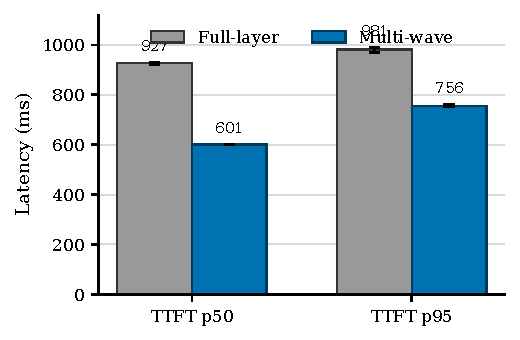
\includegraphics[width=\columnwidth]{figures/matched_ttft.pdf}
  \caption{Capacity-bounded multi-wave staging reduces the repeat-median TTFT
  p50 by 35.21\% and TTFT p95 by 22.96\% relative to graph-compatible
  full-layer staging. Bars show the median of three independent service-start
  summaries; whiskers show their minimum and maximum. The comparison uses one
  Ascend 910B2, Qwen3-30B-A3B BF16, a 14-GiB offload target, 32 slots, and
  concurrency one.}
  \label{fig:matched-ttft}
\end{figure}

\begin{table}[t]
  \centering
  \small
  \caption{Matched full-layer and multi-wave results. Each arm aggregates
  three fresh starts and 600 ShareGPT requests. Latency entries are the median
  of the three repeat-level quantiles.}
  \label{tab:matched}
  \begin{tabular}{lrrr}
    \toprule
    Mode & TTFT p50 & TTFT p95 & TPOT p50 \\
         & (ms) & (ms) & (ms/token) \\
    \midrule
    Full-layer & 927.06 & 980.89 & 54.33 \\
    Multi-wave & 600.65 & 755.68 & 54.42 \\
    \bottomrule
  \end{tabular}
\end{table}

As Figure~\ref{fig:matched-ttft} and Table~\ref{tab:matched} show, the
repeat-median TTFT p50 falls from 927.06 to 600.65~ms, a 35.21\% reduction.
The corresponding TTFT p95 falls from 980.89 to 755.68~ms, a 22.96\%
reduction. Pair-level p50 reductions range from 35.02\% to 35.55\%, and
pair-level p95 reductions range from 21.71\% to 23.63\%.

TPOT does not show the same reduction. Its repeat-level p50 values are
53.87/54.74/54.33~ms/token for full-layer and
55.34/54.42/53.87~ms/token for multi-wave. The supported performance
conclusion is therefore limited to time to first token in this prefill-heavy
boundary, not a decode-speedup claim. Each arm completes 600/600 requests and
76,800 output tokens. All six units produce identical token arrays, capture
and replay the graph, record zero fallback and runtime error events, release
their managed service, and return to 5\% final HBM.

\subsection{Q3: Overlap, recombination, and memory bounds}

The multi-wave stability profile contains 2,544 prefill-layer events and 9,077
waves. Every wave is issued before its compute begins. The runtime submits
6,533 next-wave prefetches before the current wave's compute and records no
late after-compute prefetch issue. Aggregate stage wait is 1,593.87~ms across
the profile, compared with 7,493.41~ms of profiled MLP time, and the maximum
per-layer stage wait is 1.27~ms. These measurements show that the intended
software-pipeline schedule executes online; they do not isolate the causal
latency contribution of overlap.

Exactness is checked separately from scheduling. Eleven trigger requests
match the full-layer oracle for serial eager multi-wave, overlapped eager
multi-wave, and overlapped graph multi-wave execution, covering 1,408 token IDs
per mode. A tensor-level check over 136 BF16 routed pairs split across five
interleaved waves is bitwise equal to the native combine. The only online
combine mode in the qualified profile is the native-recombination path.

The final memory ledger reports 13.50~GiB in the host expert store, 3.38~GiB
in persistent device slots, and 0.56~GiB in two prefill stage banks. Total
device slot and stage storage is 3.94~GiB. All 12 original expert-weight banks
are released, no wave exceeds 32 slots, and the physical 65,536-MiB device
peaks at 91\% HBM without an OOM or memory-growth failure.

